\documentclass[11pt,twoside]{report}
\usepackage{preamble}
\graphicspath{{../img/cha2/}}
\setcounter{chapter}{0}
\renewcommand{\chaptername}{Appendix}
\renewcommand{\thechapter}{\Alph{chapter}}

\begin{document}

\chapter{Alternative 2D Image Analysis Methods}
\label{chapter:extra-2d}

%\epigraph{Talk is cheap, show me the code.}{Linus Torvalds, 2000}

\section{Introduction}

It is possible to get information about the collective behaviour of zebrafish in a quasi-2D environment, without locating each fish individual or linking coordinates into trajectories.
We will briefly describe a ``tracking-free'' analysis and relevant results in this chapter.
The experimental setup used to observe the fish is identical to the one discussed in chapter~\ref{chapter:fish_2d}.

This tracking-free method is helpful when the fish are very densely packed, since the tracking would fail because of the constant visual occlusion.
The densely packed situation happens, as a group of fish exhibit the coexistence between dense regions and dilute regions in certain conditions. Such a ``phase-separation'' scenario is shown in Fig.~\ref{fig:mips}, where the dense regions are outlined.
This coexistence is reminiscent of the \emph{mobility induced phase separation} (\gls{MIPS}) phenomenon, commonly seen in a repulsion-dominated active matter system (chapter~\ref{chapter:collective_behaviour}) \cite{cates2015}.

\marginpar{
\centering
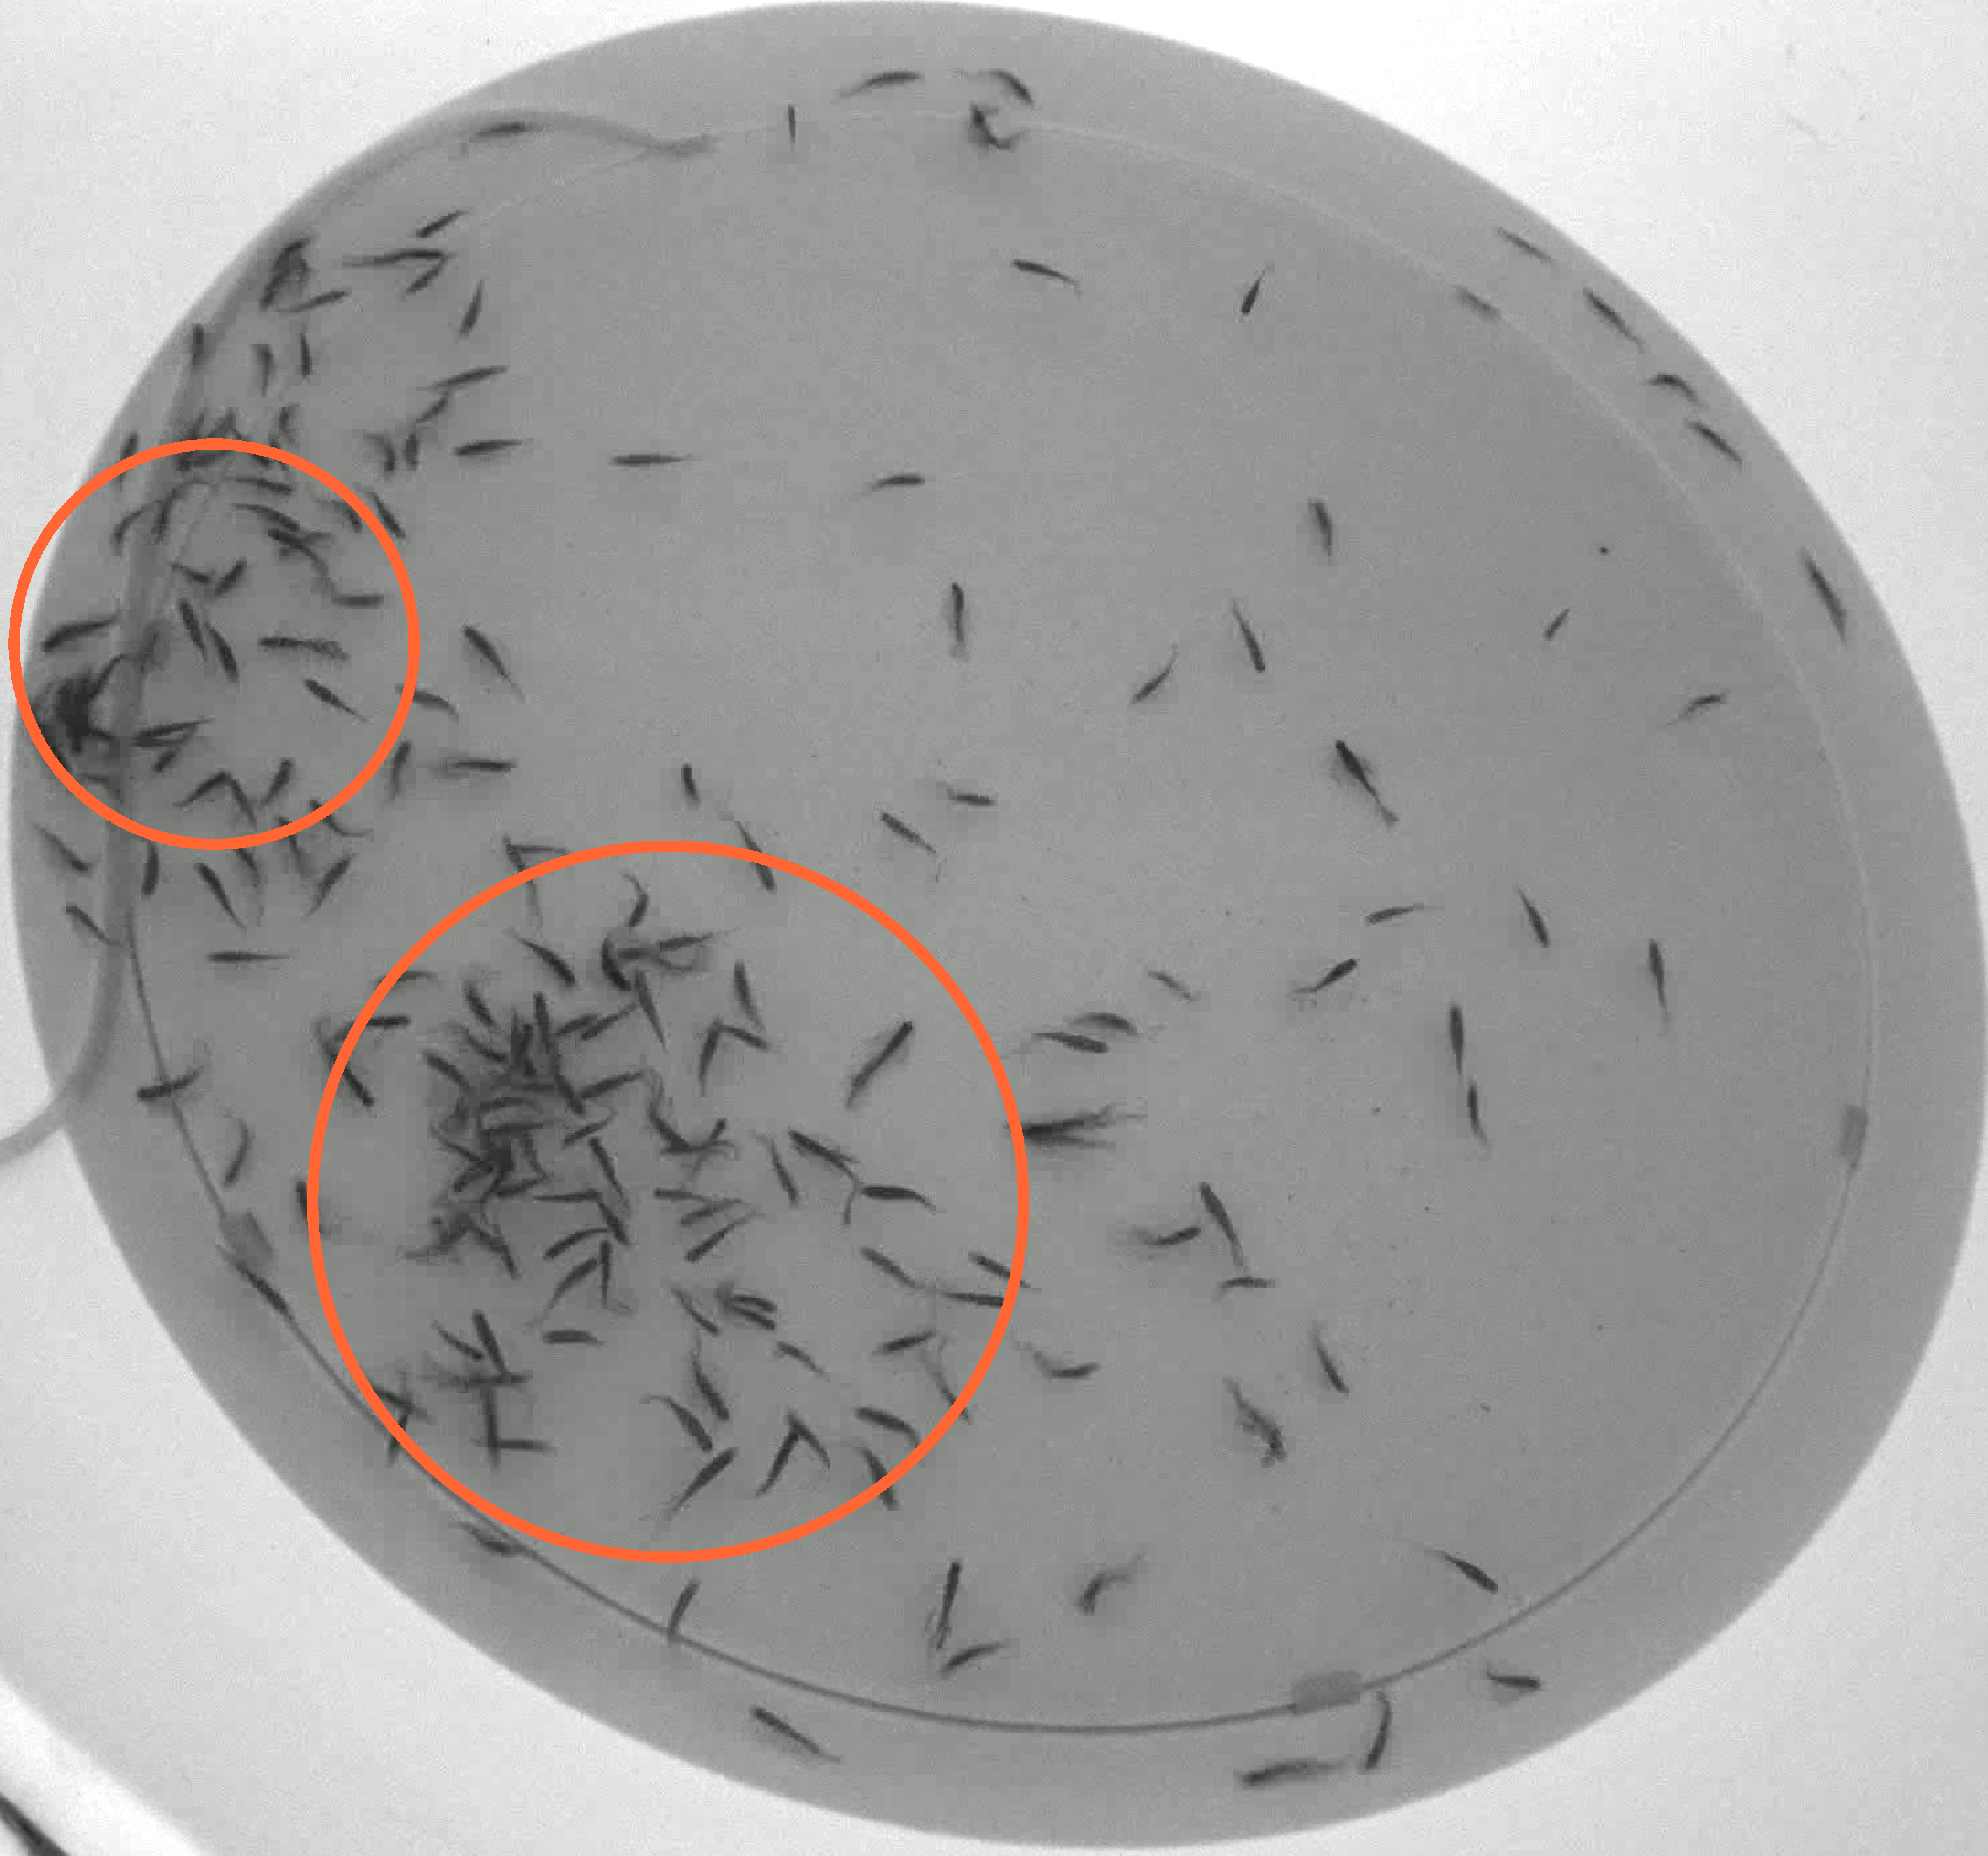
\includegraphics[width=\marginparwidth]{mips}
\captionof{figure}[Dense regions in a group of fish]{
  The dense and dilute regions in a group of fish. The group size is 200, and the fish were confined in a quasi-2D environment.
}
\label{fig:mips}
}

\section{Estimating Density Heterogeneity}



We can quantify the coexistence of the high-density ``liquid'' and low-density ``gas'' with the heterogeneity of the density distribution.
To do so, we subdivide the image into different grids with the same are, and measure the brightness variation among the grids.
One example of these grids\marginfootnote{
The areas of the grids seems different because of the projective transformation during the formation of the image. The areas are the same in the rectified image.
} is shown in Fig.~\ref{fig:density}.
For a uniformly distributed fish group, the variation would be close to zero. For phase-separated fish group, the variation would have a large value. 
Operationally, We take the sum of bright pixels in the foreground movie \gls{fijt} in each grid, as a measure of the \emph{density}, noted as $\tilde{\rho}$. We take the standard deviation of $\tilde{\rho}$ values from all grids, as a measure of the density heterogeneity, noted as $\mathcal{D} = \mathrm{std}(\tilde\rho)$.


Figure~\ref{fig:density} shows the measured \gls{dh} for 100 zebrafish. The grids were shown in Fig.~\ref{fig:density} (c), and clearly different grids have different $\tilde{\rho}$ values. The temporal evolution of $\mathcal{D}$ is shown in Fig.~\ref{fig:density} (a). We carefully kept the illumination condition in the observation room constant, to avoid sudden changes in $\mathcal{D}$. Figure~\ref{fig:density} shows the probability density function of $\mathcal{D}$, exhibiting a single peak around 1.1.


\begin{SCfigure}
  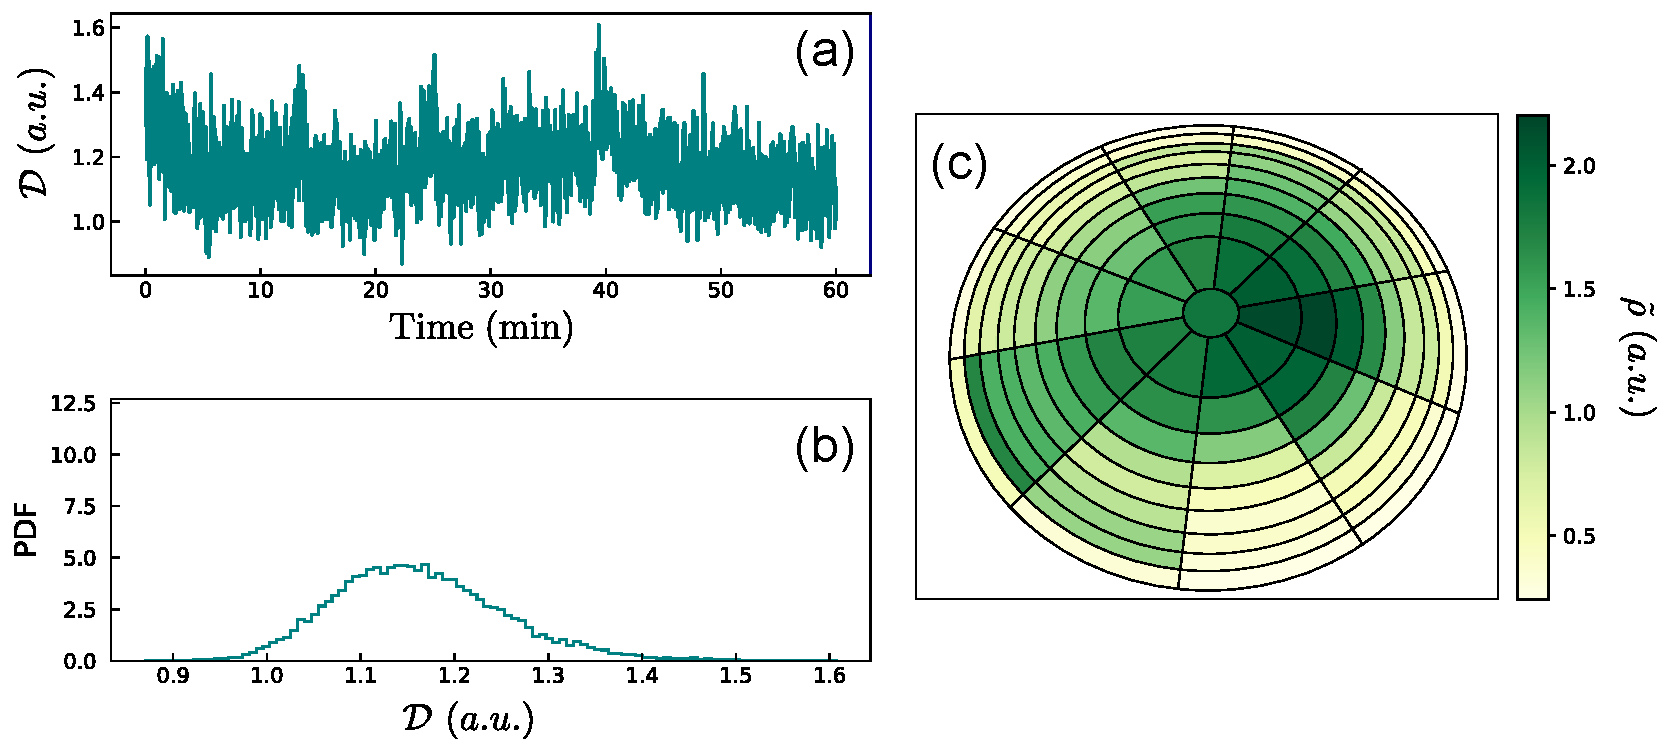
\includegraphics[width=\linewidth]{density}
  \caption[Density Heterogeneity analysis of 100 zebrafish]{
  Density Heterogeneity analysis of 100 zebrafish swimming in a quasi-2D environment. The units for $\tilde{\rho}$ and $\mathcal{D}$ are arbitrary, which are related to the pixel intensity in the image.
  (a) The density heterogeneity $\mathcal{D}$ of the fish group as a function of time. 
  (b) The probability density function of the density heterogeneity $\mathcal{D}$.
  (c) A snapshot of the density distribution of the fish. The tank was partitioned into different grids with the same area. The colour indicates the pixel brightness in each grid. Darker colour = more fish.
  }
  \label{fig:density}
\end{SCfigure}




\section{Estimating the Mobility}


If we think of a group of zebrafish as active matter, we would want to measure its \emph{activity}, which controls the phase behaviour of the system. The direct measurement of the activity requires the trajectory of individual fish from tracking result. A simpler measurement is the \emph{mobility} of the fish group, which is defined as

\begin{equation}
	\mathcal{M} = \sum_{ij}\left\vert F_{ij}(t + 1) - F_{ij}(t) \right\vert,
\label{eq:mobility}
\end{equation}

\noindent where $F_{ij}(t)$ represents the pixel value of the foreground video at time $t$ (see section~\ref{section:image_process} for details).

Figure~\ref{fig:mobility} shows the measured $\mathcal{M}$ for 100 zebrafish. The different between two success frames in the foreground video, $\Delta F_{ij}(t)$, is shown in Fig.~\ref{fig:mobility} (c), whose absolute sum is the mobility. The values of \gls{mob} as a function of time is plotted in Fig.~\ref{fig:mobility} (a). The probability density function of $\mathcal{M}$ is shown in Fig.~\ref{fig:mobility} (b), featuring a single peak.

\begin{SCfigure}
  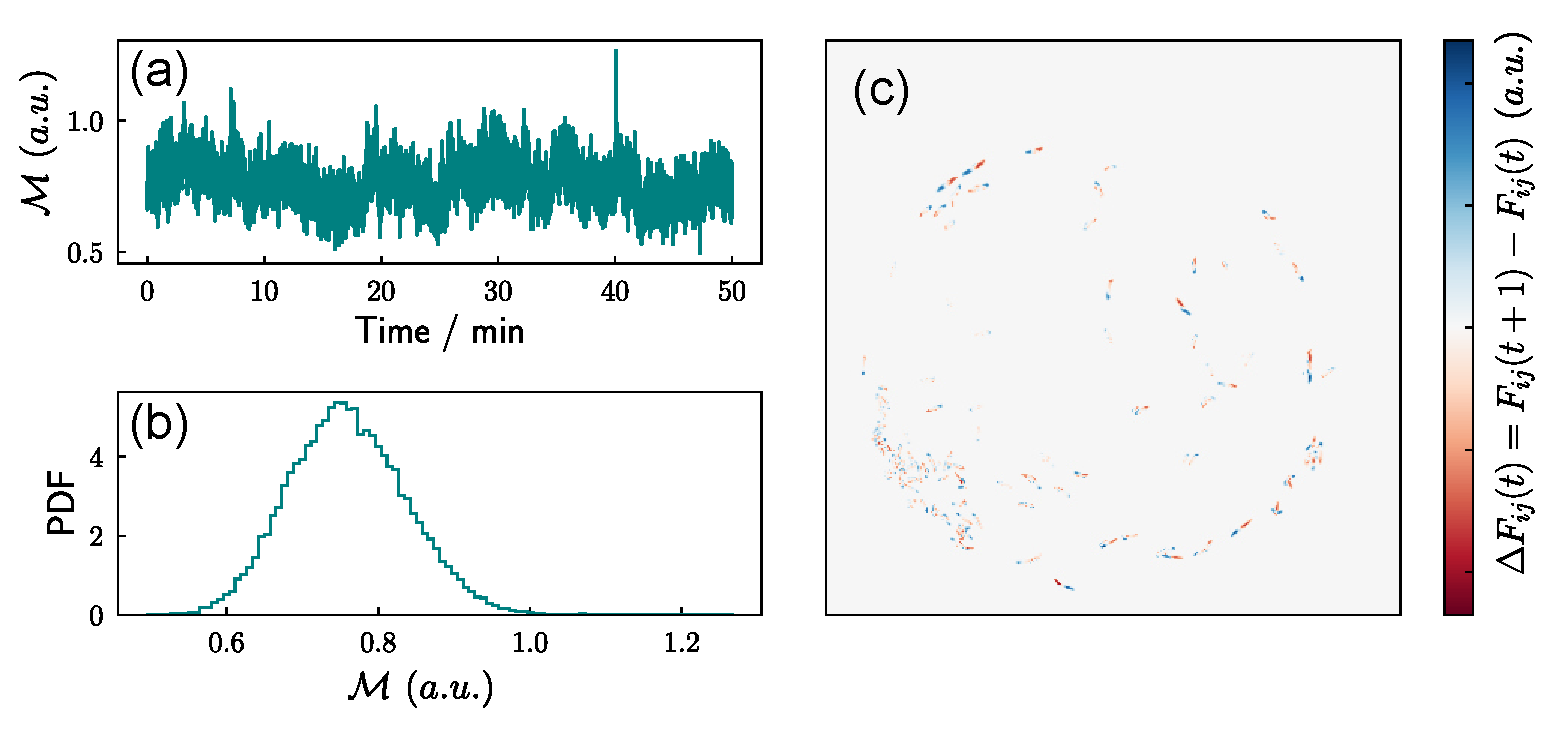
\includegraphics[width=\linewidth]{mobility}
  \caption[The mobility analysis of 100 zebrafish]{
  The mobility analysis of 100 zebrafish swimming in a quasi-2D environment. The unit for $\mathcal{M}$ is arbitrary, which is related to the pixel intensity in the image.
  (a) The mobility $\mathcal{M}$ of the fish group as a function of time. 
  (b) The probability density function of the mobility $\mathcal{M}$.
  (c) The difference between two success frames. The dark pixels contains the moving fish.
  }
  \label{fig:mobility}
\end{SCfigure}

\section{Changing States of the Fish Group}

We changed the macroscopic state of the fish, by applying different illumination conditions with a smart bulb. It was expected that the fish would perceive more danger in a brighter environment, which leads to a higher $\mathcal{D}$ value for the group. However, we found that the fish group have non-monotonic response to the brightness of the environment.

The changing macroscopic states of different fish groups, with different group sizes, is shown in Fig.~\ref{fig:brightness}. It is not clear how increasing the brightness level would change the $\mathcal{D}$ and $\mathcal{M}$ values of the fish group. The absence of a monotonic relationship could be the result of the other biological or environmental factors, which requires more studies in the future.

However, it is clear that the fish groups exhibited very different macroscopic states, under different illumination conditions. These changing states is consistent with our analysis in chapter~\ref{chapter:fish_analysis}.

\begin{SCfigure}
  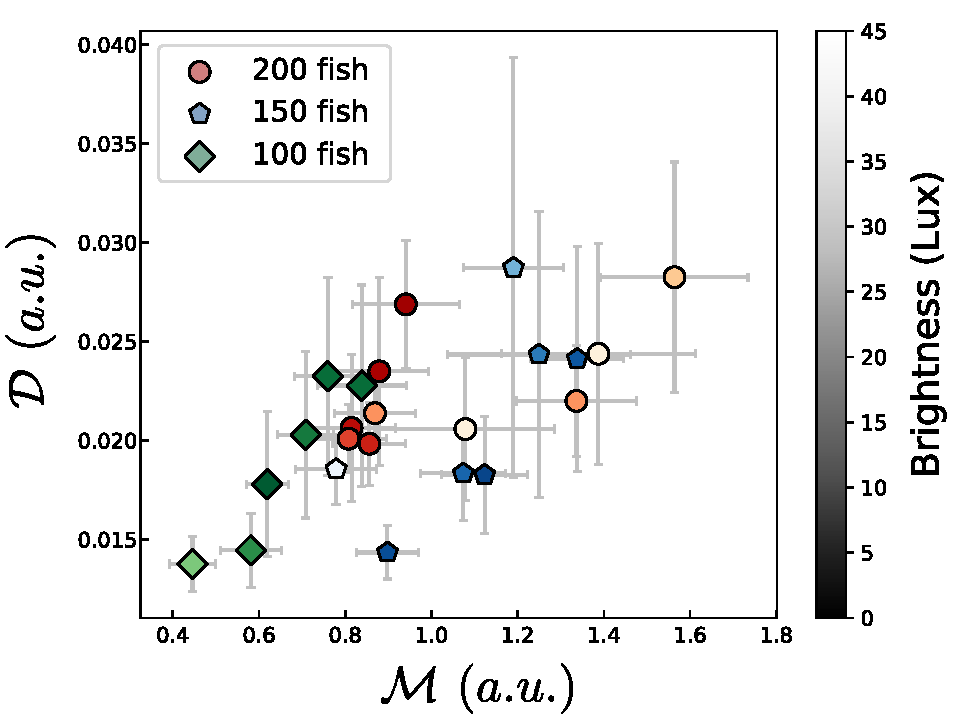
\includegraphics[width=\linewidth]{brightness}
  \caption[The changing macroscopic states of zebrafish]{
  The changing macroscopic states of zebrafish under different illumination conditions. The macroscopic state is indicated by the density heterogeneity ($\mathcal{D}$) and the mobility ($\mathcal{M}$) of the fish group. The error bars represent the standard error of the measurement.
  }
  \label{fig:brightness}
\end{SCfigure}

\section{MIPS as a Possible Explanation}

The different density heterogeneity $\mathcal{D}$ and mobility $\mathcal{M}$ values of the fish group could be understood as a MIPS-like behaviour (chapter~\ref{chapter:collective_behaviour}). The result is organised in Fig.~\ref{fig:phase-mips}, where we use the value of $\mathcal{D} / N$ as the order parameter. 
A large $\mathcal{D} / N$ value indicates the coexistence of a dense phase and a dilute phase, therefore the MIPS.

For the observed fish groups, the MIPS-like behaviour happened if the mobility per fish ($\mathcal{M}/N$, as a proxy to the \emph{activity}) is large, and the fish number (as a proxy to the \emph{density}) is moderate. This is in-accordance of the phase behaviour of repulsion dominated active matter systems (for instance the active Brownian particles) \cite{turci2021}.

However, the emergence of MIPS-like behaviour for a group of fish is a surprising result, which needs more careful studies. For instance, more state points should be sampled in the phase diagram. In addition, more detailed analysis is needed. For instance, one should check if the dense regions are also slow, as a result of the feedback loop in MIPS. Finally, the ``tracking-free'' analysis in this chapter is novel, which needs validation. For instance, we should compare the results of this tracking-free analysis, with the results from widely accepted analysis based on tracking individuals.

\begin{SCfigure}
  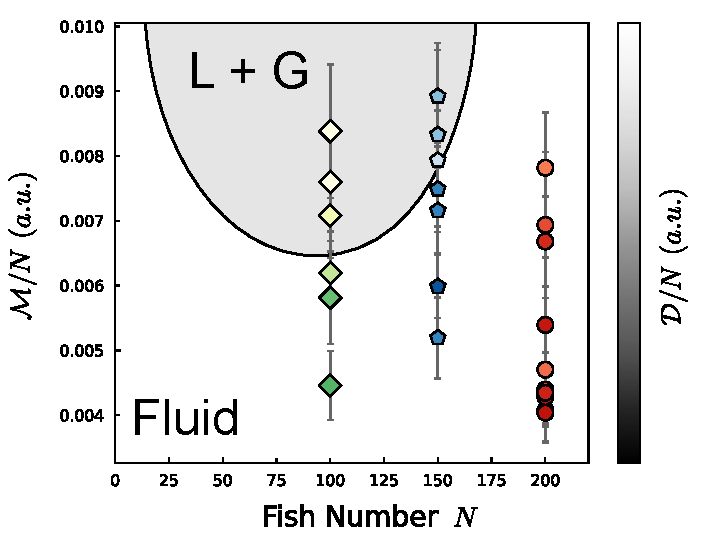
\includegraphics[width=\linewidth]{phase}
  \caption[MIPS like phase behaviour of zebrafish]{
  The changing macroscopic states of zebrafish exhibiting a MIPS like phase behaviour. The fish number (\gls{N}) is related to the density, and the mobility divided by the fish number ($\mathcal{M}/N$) is a proxy to the activity. In a high activity and moderate density region, we observe a high density heterogeneity per fish ($\mathcal{D}/N$) value, corresponding to the coexistence of a dense phase (liquid) and a dilute phase (gas). The coexistence region is drawn manually for illustration.
  }
  \label{fig:phase-mips}
\end{SCfigure}

\vfill

\begin{adjustwidth}{0cm}{-5cm}
\begin{tcolorbox}[
fonttitle=\sffamily\Large,
right=0.1\linewidth,
top=5mm,
bottom=5mm,
title=Summary of Appendix A,
]

\begin{itemize}
	\item We proposed a new method to analyse the video for a group of fish in a quasi-2D environment, with out tracking the movement of the individuals.
	\item The density heterogeneity of the fish group can be estimated by subdividing the image into grids, and calculating the intensity variation in different grids.
	\item The mobility of the fish group can be estimated by the difference between two successive frames.
	\item The changing illumination condition changed the macroscopic states of the fish group. But the fish respond to the changing brightness level in a non-monotonic way.
	\item The different macroscopic states of the fish group is similar to the MIPS behaviour of repulsion-dominated active particles.
\end{itemize}
\end{tcolorbox}

\end{adjustwidth}

\end{document}
